% Motivação ----------------------------------------------------------
\section{Motivação}

\begin{frame}{ML é ótimo para associações}
	\textbf{ML tradicional é excelente em perguntas como:}
	\begin{center}
		\Large \emph{``O que costuma acontecer junto de X?''}
	\end{center}
	\vfill
	\pause
	Mas não é tão eficaz para perguntas do tipo:
	\begin{itemize}
		\item \textbf{``O que acontece se eu intervir?''} --- \emph{do}(X)
		\item \textbf{``Quais atributos realmente causam esse resultado?''}
		\item \textbf{``O que precisaria mudar para o resultado ser diferente?''}
	\end{itemize}
\end{frame}

\begin{frame}{Associação $\neq$ Intervenção}
	\begin{block}{Um exemplo clássico}
		Alarmes de incêndio estão fortemente correlacionados com a presença de bombeiros no local.
	\end{block}
	\pause
	\begin{alertblock}{Intervenção é outra coisa}
		Instalar mais alarmes (\emph{do}(alarme = ligado)) não traz mais bombeiros.
	\end{alertblock}
	\pause
	\centering \textbf{$P(Y \mid X) \neq P(Y \mid do(X))$}
\end{frame}

\begin{frame}{Correlação $\neq$ Causalidade}
	\centering
	{\large Nicolas Cage causa afogamentos?}
	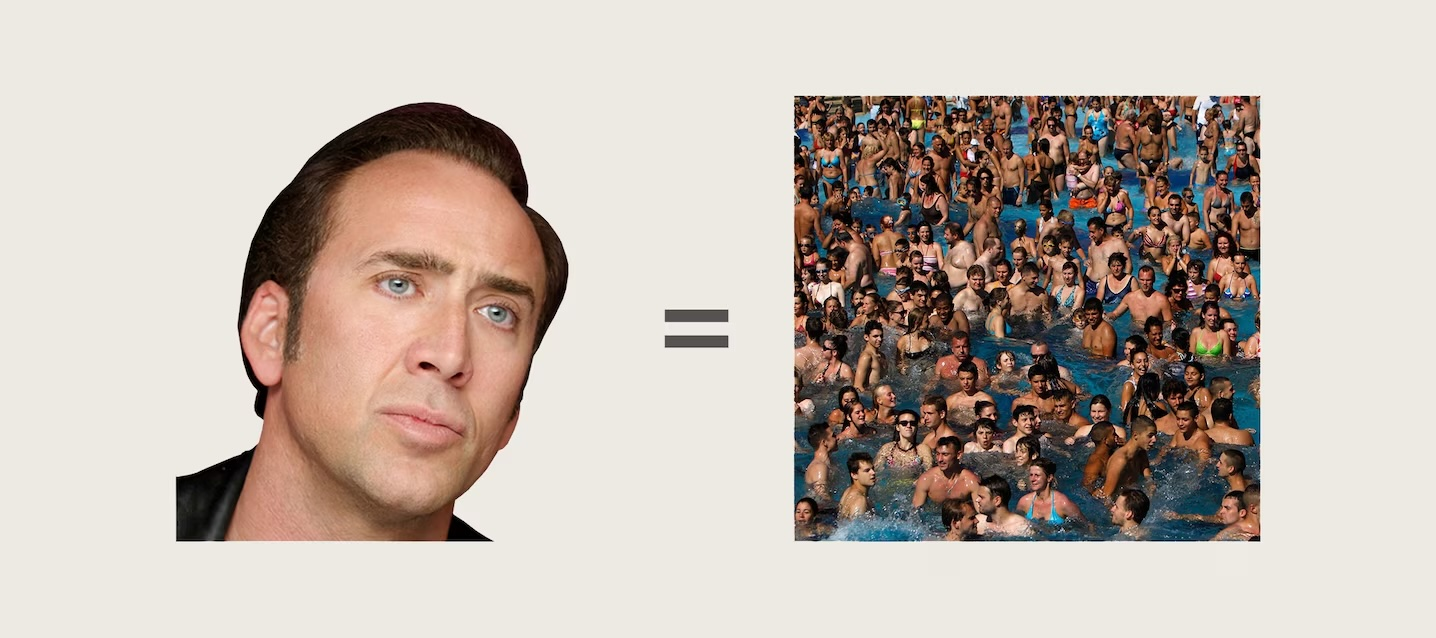
\includegraphics[width=\linewidth]{figures/nicolas_cage_drowning.jpg}
\end{frame}
\begin{frame}{Correlação $\neq$ Causalidade}
	\centering
	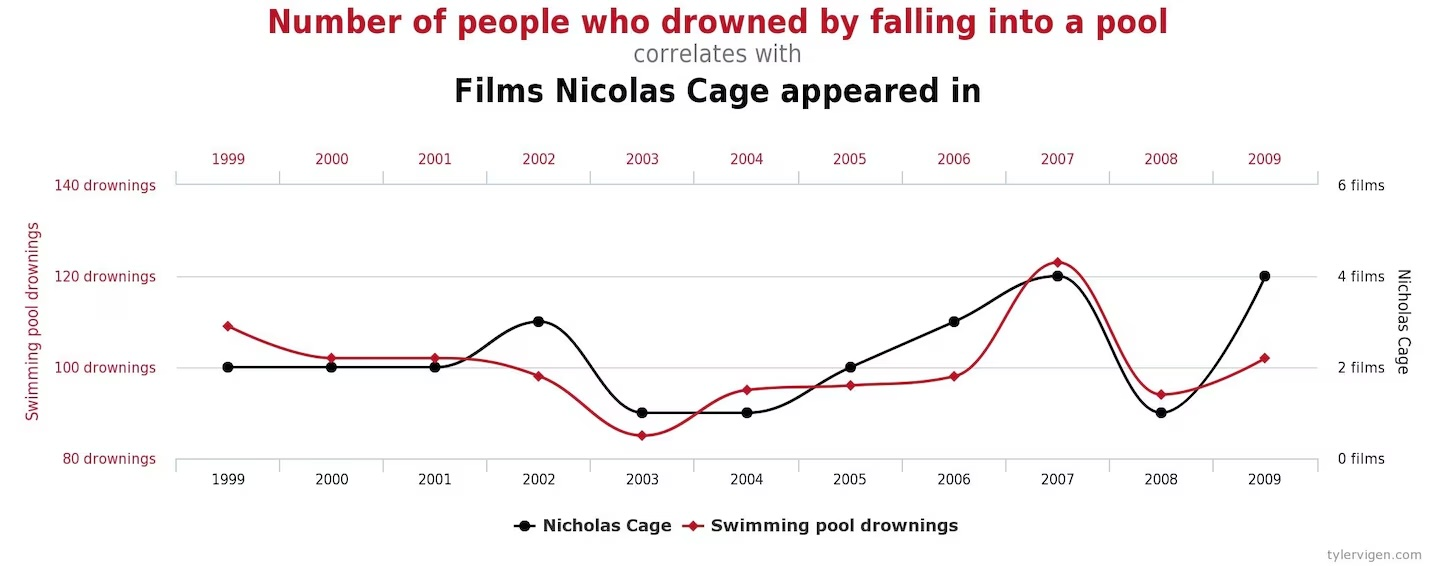
\includegraphics[width=\linewidth]{figures/nicolas_cage_drowning_2.jpg}
\end{frame}

\begin{frame}{... e o que isso tem a ver com ciência de dados?}
	Duas variáveis podem ter uma associação em um sentido na população inteira, e no sentido oposto em \emph{cada} subgrupo.
	\pause
	\vfill
	Esse cenário não é muito raro, e é consequência direta de confundimento (\emph{confounding}). 

	Vamos ver?
\end{frame}

\subsection{Paradoxo de Simpson}

% \begin{frame}{Paradoxo de Simpson}
% 	\textbf{Planejado (plan.md 4.1):}
% 	\begin{itemize}
% 		\item Limitações do ML tradicional: associação vs. intervenção
% 		\item Estudo de caso: vacinação COVID-19 (Reino Unido)
% 		\item Reversão de tendência por subgrupo (idade)
% 	\end{itemize}
% \end{frame}

\begin{frame}{Mão na massa}
	\notebooklink{1}{1\_simpsons\_paradox\_example.ipynb}
\end{frame}


